\section{Domain Theory}
There is an entire area of mathematics devoted to exploring these structures called \emph{Domain Theory}, as described in \citep{Gunter92} and  \citep{Hutton14}.

We define domains by using \emph{chains}. Another way of defining domain is with directed sets, as all chains are directed sets.

A \emph{chain} is a sequence $x_0 \sqsubseteq x_1 \sqsubseteq x_2 \sqsubseteq \dots $ where every element is larger than the preceding one.

Formally we define a chain as a function $\mathbb{N} \to X$, such that if $i \leq j$ then $x_i \sqsubseteq x_j$

As an example, given the lifted set  $\natb$ (a set with $\bot$ added) then a chain can be formed in three ways:

\begin{itemize}
\item{$\bot \sqsubseteq \dots \sqsubseteq \bot$, for any number of $\bot$s}
\item{$n \sqsubseteq \dots \sqsubseteq n$, for any number of $n$ , where $n$ is the same number each time}
\item{$\bot \sqsubseteq \dots \sqsubseteq \bot \sqsubseteq n \sqsubseteq \dots \sqsubseteq n$, for any number of $\bot$s followed by any number of identical $n$s}
\end{itemize} 

\section{Definition of a domain}
A domain is a set $X$, an element $\bot \in X$ and a relation $\sqsubseteq \ \subseteq X \times X$ such that:

\begin{itemize}
\item{$\forall x \in X. \ \bot \sqsubseteq X$}
\item{$\sqsubseteq$ is a partial order}
\item{All chains of elements of $X$ have a limit. To prove this there are two properties we must prove, for some $z \in X$}
\begin{itemize}
 \item{$\forall i. x_i \sqsubseteq z$ \hspace{1cm} \emph{($z$ is the upper bound)}}
 \item{$\forall y. (\forall i.x_i  \sqsubseteq y) \Rightarrow \ z \sqsubseteq y$ \hspace{0.25cm} \emph{($z$ is the least upper bound)}}
\end{itemize}
\end{itemize}

%\textcolor{red}{EXPLAIN WHY LIMIT NEEDED}

\section{Examples of Domains}
\subsection{Single Element Domain}
In a single element domain we have the set $\{x\}$, so $\bot = x$ and $\sqsubseteq$ just contains $(x,x)$

Now we must prove three conditions to show that $(\{x\},\sqsubseteq)$ is a domain).

\begin{enumerate}
\item{$\forall x \in \{x\}. x \sqsubseteq x$\\
There is only one element, $x$ and $x \sqsubseteq x$ is in the ordering.}
\item{$\sqsubseteq$ \textbf{is a partial order}
\begin{itemize}
\item{Reflexivity\\
The only element is $x$ and $x \sqsubseteq x$ is in the ordering}
\item{Antisymmetry\\
 $x,y$ must both be $x$, as it is the only possible element, so $x = x$.}
\item{Transitivity\\
 $x,y$ and $z$ must all be $x$ and $x \sqsubseteq x$ is in the ordering.}
\end{itemize}}
\item{\textbf{All chains must have a least upper bound}\\
As $x$ is the only possible element, all chains will be of the form 

\[ x \sqsubseteq x  \sqsubseteq x  \sqsubseteq \dots \]

Therefore we define $\sqcup \{x\} = x$.

Then we need an element $z$ such that the following two statments are true. Let $z = \sqcup\{x\} = x$. Then:

\begin{itemize}
\item{$\mathbf{\forall i. x_i \sqsubseteq z}$ \\
The only possible $x_i$ is $x$, so we must have $x \sqsubseteq x$. This is in the ordering.}
\item{$\mathbf{\forall y. (\forall i . x_i \sqsubseteq y) \Rightarrow z \sqsubseteq y}$\\
The only possible value of $y$ is $x$. Therefore we must have $x \sqsubseteq x$, which is in the ordering.}
\end{itemize}}
\end{enumerate}

\vspace{0.25cm}

Now we have proved all the conditions, so the single element domain is a domain.


\subsection{Flat Natural Numbers} A \textbf{flat} domain is a special kind of domain where the only ordering is between $\bot$ and the elements of the set. In this example the set is  $\mathbb{N}$, the set of natural numbers:

In our domain, the set $X = \mathbb{N}_\bot$, so we have each number and a bottom element, $\bot$ that carries less information than a number. The only orderings we have are $\bot \sqsubseteq 0$, $\bot \sqsubseteq 1$, $\bot \sqsubseteq 2$, etc..., so the relation is defined as:

\[ \sqsubseteq  \ = \{ (\bot , \bot) \} \cup \{ (\bot , n) , (n ,n) \ | \ n \in \mathbb{N} \} \] 

which gives us the following picture:   

\vspace{0.5cm}

\begin{center}
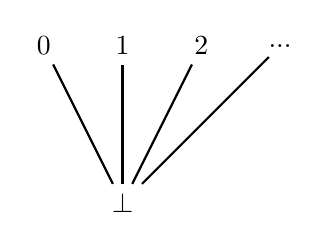
\begin{tikzpicture}
    \node (top) at (0,0) {$\bot$};
    \node (a) at (-1,2) {0};
    \node (b) at (0,2) {1};
    \node (c) at (1,2) {2};
    \node (d) at (2,2) {...};
    \draw [thick] (top) -- (a);
    \draw [thick] (top) -- (b);
    \draw [thick] (top) -- (c);
    \draw [thick] (top) -- (d);
\end{tikzpicture}
\end{center}

\vspace{0.5cm}

Now we must prove three conditions to show $(\mathbb{N}_\bot, \sqsubseteq)$ is a domain: 

\begin{enumerate}
\item{$\forall x \in \natb. \ \bot \sqsubseteq x$ }\\
In the definition of our relation we have $\{ (\bot , n) \ | \ n \in \mathbb{N} \}$ and $(\bot , \bot)$. so $\{(\bot , x) \ | x \in \natb\}$ is a subset of $\sqsubseteq$.
\item{\textbf{Prove $\sqsubseteq$ is a partial order}\\
For $\sqsubseteq$ to be a partial order, it must be reflexive, antisymmetric and transitive.
\begin{itemize}
\item{Reflexivity\\
$\sqsubseteq$ is \emph{reflexive} by definition, as we have $\{(x,x) \ | \ x \in \natb \}$ as a subset of $\sqsubseteq$.}
\item{Antisymmetry\\
When $x = \bot$, the only possible $y$ we can have such that $y \sqsubseteq x$, is $y = \bot$, as  $n \sqsubseteq \bot$ is not defined in the relation for any $n$. Therefore $x = y = \bot$.

When $x = n$, the only possible value of $y$ is $n$, so $x = y = n$.

Therefore $\sqsubseteq$ is \emph{antisymmetric}}
\item{Transitivity \\
If $x = \bot$, a possibility for $y$ is $y =n$. Then we must have $z = n$ for $(y,z)$ to be in $\sqsubseteq$. Then we need $\bot \sqsubseteq n$ , which we have, as we have $(\bot, n)$, for any $n \in \mathbb{N}$, defined in the relation. $y$ could have also been $\bot$. Then we have both options for $z$. When $z = n$, we should have $\bot \sqsubseteq n$, which we have, as we have $(\bot, n)$ for any $n \in \mathbb{N}$ defined in the relation. When $z = \bot$, we just want $ \bot \sqsubseteq \bot$, which is also in the definition of $\sqsubseteq$.

If $x = n$, then both $y$ and $z$ must also be equal to $n$ for $x \sqsubseteq y$ and $y \sqsubseteq z$ to be defined. Therefore we should  have $n \sqsubseteq n$. This is in the definition of $\sqsubseteq$.

Therefore $\sqsubseteq$ is \emph{transitive}.}
\end{itemize}}

\item{\textbf{All chains must have a least upper bound}\\

For any chain of elements of $\mathbb{N}_\bot$, we must prove there exists a $z \in \natb$ satisfying the two statements. We must prove two statements, by case analysis on the different chains:

\begin{enumerate}
\item{$\bot \sqsubseteq \dots \sqsubseteq \bot$\\ 
For these chains, we never have any numbers, so $z = \bot$. The last element in the chain will always be $\bot$, so for every $i$ we have $\bot \sqsubseteq \bot$. Therefore $\forall i . x_i \sqsubseteq \bot$.
For the second statement, as every element is $\bot$,$x_i = \bot$ and $y = \bot$, we have $\bot \sqsubseteq \bot$ for $z \sqsubseteq y$. Therefore $\forall y. (\forall i . x_i \sqsubseteq y) \Rightarrow \bot \sqsubseteq y$ holds.}
\item{$n \sqsubseteq \dots \sqsubseteq n$ \\
 For the chains just containing $n$, let $z = n$. The last element in the chain will always be $n$, so for every $n$ we have $n \sqsubseteq n$. Therefore $\forall i . x_i \sqsubseteq n$.

For the second part, every element is $n$, so $x_i = n$ and $y = n$. Then we have $n \sqsubseteq n$ for $z \sqsubseteq y$. Therefore $\forall y. (\forall i . x_i \sqsubseteq y) \Rightarrow n \sqsubseteq y$ holds.}
\item{$\bot \sqsubseteq \dots \sqsubseteq \bot \sqsubseteq n \sqsubseteq \dots \sqsubseteq n$\\
For these chains, let $z = n$.  The last element will be $n$. We have both $\bot \sqsubseteq n$ and $n \sqsubseteq n$ in the relation, so for any $x$, we have $x \sqsubseteq n$. Therefore $\forall i . x_i \sqsubseteq n$.

For the second part, $(\forall i . x_i \sqsubseteq y)$ is only true when $y = n$, so we only have to consider this case. Then we have $n \sqsubseteq n$ for $z \sqsubseteq y$. Therefore $\forall y. (\forall i . x_i \sqsubseteq y) \Rightarrow n \sqsubseteq y$ holds.}
\end{enumerate}}
\end{enumerate}

\subsection{Product of domains}
\section{Product of Domains}
Given two domains $\mathbb{X} = X, \bot_X, \sqsubseteq_X$ and $\mathbb{Y} = Y, \bot_Y, \leq_Y$, we have the following:

\begin{itemize}
\item{$X \times Y$ is the set}
\item{$\bot = (\bot_X, \bot_Y)$}
\item{$(x,y) \sqsubseteq (x',y')$ is defined when $x \sqsubseteq_X x'$ and $y \leq_Y y'$ are defined}
\end{itemize}

\subsection{$\forall (x,y) \in X \times Y. \bot  \sqsubseteq (x,y)$}
Because $\mathbb{X}$ is a domain, we know $\forall x \in X. \bot_X \sqsubseteq_X x$.
Because $\mathbb{Y}$ is a domain, we know $\forall y \in Y. \bot_Y \leq_Y y$.

Therefore we have $\forall x,y . \bot_X \sqsubseteq_X x \wedge \bot_Y \leq_Y y$. This is the same as $\forall (x,y) \in X \times Y. (\bot_X,\bot_Y) \sqsubseteq (x,y)$

\subsection{$\sqsubseteq $ is a partial order}

\paragraph{Reflexivity} For an element $(x,y) \in X \times Y$, we have $x \sqsubseteq_X x$ and $y \leq_Y y$ because $\mathbb{X}$ and $\mathbb{Y}$ are domains, so their orderings are reflexive. This means we have $(x,y) \sqsubseteq (x,y)$.

\paragraph{Antisymmetry} For elements $(x,y)$ and $(x',y')$ we can assume $(x,y) \sqsubseteq (x',y')$ and $(x',y') \sqsubseteq (x,y)$. Expanding these definitions we have $x \sqsubseteq_X x' \wedge y \leq_Y y' \wedge x' \sqsubseteq_X x \wedge y' \leq_Y y$. If we reorder this we have:

\[x \sqsubseteq_X x' \wedge x' \sqsubseteq_X x \wedge y \leq_Y y' \wedge y' \leq_Y y \]

As the orderings on $\mathbb{X}$ and $\mathbb{Y}$ are antisymmetric, we can rewrite this as $x = x'$ and $y = y'$. Therefore we have $(x,y) = (x',y')$.

\paragraph{Transitivity} For elements $(x,y), (x',y')$ and $(x'',y'')$ we can assume $(x,y) \sqsubseteq (x',y')$ and $(x',y') \sqsubseteq (x'',y'')$. Expanding these definitions we have $x \sqsubseteq_X x' \wedge y \leq_Y y' \wedge x' \sqsubseteq_X x'' \wedge y' \leq_Y y''$. If we reorder this we have:


\[x \sqsubseteq_X x' \wedge x' \sqsubseteq_X x'' \wedge y \leq_Y y' \wedge y' \leq_Y y'' \]

As the orderings on $\mathbb{X}$ and $\mathbb{Y}$ are transitive, we can rewrite this as $x \sqsubseteq_X x''$ and $y \leq_Y y''$. Therefore we can now define $(x,y) \sqsubseteq (x'',y'')$.

\subsection{All chains have a least upper bound}
Chains of $X \times Y$ will be of the form:

\[(x,y) \sqsubseteq (x', y') \sqsubseteq (x'', y'') \sqsubseteq \dots \]

where $x \sqsubseteq_X x' \sqsubseteq_X x'' \dots$ and $y \leq_Y y' \leq_Y y'' \dots $.

Then we need an element $z$ such that the following two statements are true. Let $z = \sqcup (x_i, y_i) = (\sqcup x_i, \sqcup y_i)$. Then:

\begin{itemize}
\item{$\mathbf{\exists z \in X \times Y . \forall i. (x_i, y_i) \sqsubseteq z}$ \\
As $\mathbb{X}$ and $\mathbb{Y}$ are domains, we have $\forall i. x_i \sqsubseteq_X \sqcup x_i$ and  $\forall i. y_i \leq_Y \sqcup y_i$. Therefore, for any $(x,y)$ we have $\forall i. (x_i ,y_i) \sqsubseteq (\sqcup x_i , \sqcup y_i)$.}
\item{$\mathbf{\exists z \in X \times Y . \forall (x',y'). (\forall i . (x_i,y_i) \sqsubseteq (x',y')) \Rightarrow z \sqsubseteq (x',y')}$\\
As $\mathbb{X}$ and $\mathbb{Y}$ are domains, we have $\forall x'. (\forall i. x_i \sqsubseteq_X x') \Rightarrow \sqcup x_i \sqsubseteq_X x'$ and $\forall y'. (\forall i. y_i \leq_Y y') \Rightarrow \sqcup y_i \leq_Y y'$.}
\end{itemize}

 Therefore if we assume $\forall (x',y'). (\forall i . (x_i,y_i) \sqsubseteq (x',y'))$, then we know $\sqcup x_i \sqsubseteq_X x'$ and $\sqcup y_i \leq_Y y'$. This is the definition of $(\sqcup x_i , \sqcup y_i) \sqsubseteq (x',y')$.

\vspace{0.25cm}

Now we have proved all the conditions, so the product of two domains is also a domain.

\section{Continuous Functions}

Given two domains, $\mathbb{X} = (X, \bot_X, \sqsubseteq_X)$ and $\mathbb{Y} = (Y, \bot_Y, \leq_y)$ The set $Cont(X,Y) =\{ f : X \to Y\}$ where:

\begin{itemize}
\item{$\forall x, x' \in X. \ x \sqsubseteq_X x' \Rightarrow f(x) \leq_Y f(x')$}
\item{$x \in Chain(X) \Rightarrow f(\sqcup x_i) = \sqcup f(x_i)$}
\end{itemize} 

The relation $\rel$ is defined as

\[ \rel  \ = \{ (f , g) \ | f,g \in Cont(X,Y) \ \wedge \ \forall x \in X. \ f(x) \leq_Y g(x)\} \]

\section{$\forall f \in Cont(X,Y). \ \bot \rel f$ }
$\bot_{X \to Y}$ is defined as the function $\bot = \lambda x. \bot (x)$, the function that loops on all inputs. The output of this function will always be $\bot$, because it does not terminate.  So for all $x \in X$ we have $\bot \leq_Y f(x)$. As $\mathbb{Y}$ is a domain we know this holds for every element of $Y$ and as the codomain of $f$ is $Y$, every $f(x)$ is in $Y$. Therefore $\bot \rel f$.
\section{Prove $\rel$ is a partial order}
For $\rel$ to be a partial order, it must be reflexive, antisymmetric and transitive. As $\mathbb{Y}$ is a domain, we know that $\leq_Y$ is a partial order.

\paragraph{Reflexivity}
We need to prove that $\forall f \in Cont(X,Y). \ f \rel f$. We can rewrite this using the definition of $\rel$ to get 
\[\forall f \in Cont(X,Y). \ (\forall x \in X. \ f(x) \leq_Y f(x))\]
 Functions are single valued, so we know $\forall f. \forall x. \ f(x) = f(x)$ and as $\leq_Y$ is reflexive we know $\forall f. \forall x \in X. \ f(x) \leq_Y f(x)$. Therefore we have $f \rel f$, for any $f \in Cont(X,Y)$. 

\paragraph{Antisymmetry}
We need to prove that $\forall f,g \in Cont(X,Y). \ f \rel g \wedge g \rel f \Rightarrow f = g$. Rewriting this using the definition of $\rel$ gives us
 \[\forall f,g \in Cont(X,Y). \ (\forall x \in X. \ f(x) \leq_Y g(x) \wedge g(x) \leq_Y f(x) \Rightarrow f(x) = g(x))\] 
 $\leq_Y$ is antisymmetric, so we have $\forall x \in X. \ f(x) = g(x)$, for any values of $f$ and $g$. Therefore $\rel$ is also antisymmetric. 


\paragraph{Transitivity}
We need to prove that $\forall f,g,h \in Cont(X,Y). \ f \rel g \wedge g \rel h \Rightarrow f \rel h$. Rewriting this using the definition of $\rel$ gives us 

\[\forall f,g,h \in Cont(X,Y). \ (\forall x \in X. \ (f(x) \leq_Y g(x) \ \wedge \ g(x) \leq_Y h(x)) \Rightarrow f(x) \rel h(x)) \]
 
As $\leq_Y$ is transitive, we have $\forall x \in X.f(x) \leq_Y h(x)$, for all $f, g$ and $h$. Therefore $\rel$ is also transitive. 

\vspace{0.7cm}

All three properties hold, so $\rel$ is a partial order on $Cont(X,Y)$

\section{All chains have a least upper bound (limit)}

For all chains $f$ in $Chain (Cont(X,Y)$), when $\exists z  \in Cont(X,Y)$ we must have:

\begin{itemize}
\item{$\forall i . f_i \rel z$}
\item{$\forall g. (\forall i . f_i \rel g) \Rightarrow z \rel g$}
\end{itemize}

Let $z = \lambda x. \sqcup^Y f_i (x)$, where $\sqcup^Y f_i (x)$ is the limit of the chain obtained by applying the functions in $Cont(X,Y)$ to a certain element $x \in X$.

A chain of functions will be a chain of elements of the set $Cont(X,Y)$, for example 

\[ f_1 \rel f_2 \rel \dots \rel \sqcup f_i \]

If we expand this using the definition of $\rel$ we have

\[ \forall x \in X. \ (f_1(x) \leq_y f_2(x) \leq_Y \dots \leq_Y \sqcup f_i (x)) \]

This is a set of chains in $Chain(\mathbb{Y})$ where every chain contains the result of each function on a certain $x$ value. As $\mathbb{Y}$ is a domain, for any chain using the elements of $Y$, rhe least upper bound is defined. Therefore we know that the least upper bound $\sqcup f_i (x)$ is defined. Now we can see that this is the same as our definition of $z$. 

\[ z = \lambda x. \sqcup^Y f_i (x)\]


For the second part of the proof, we can rewrite it using the definition of $\rel$ as

\[ \exists z \in Cont(X,Y). \  \forall x \in X. \ (\forall g. (\forall i . f_i(x) \leq_Y g(x)) \Rightarrow z(x) \leq_Y g(x)) \]


As $\mathbb{Y}$ is  a domain, $(\forall i . f_i(x) \leq_Y g(x)) \Rightarrow z(x) \leq_Y g(x))$ holds for each of our individual chains for each $x \in X$. Therefore we have $\exists z \in Cont(X,Y). \  \forall g. (\forall i . f_i \rel g) \Rightarrow z \rel g$


\vspace{0.75cm}
%
%Now we have proved that there exists a lower bound, $z$, for every possible chain, so our set $\natb $ and partial order has a least upper bound for every  chain in $Chain(\natb)$, the set of possible chains we can form with $\natb$.
%
%\vspace{0.75cm}
%We have proved that $\natb$ with the ordering $\sqsubseteq$ is a pointed poset with a least upper bound for all of its chains, so it must be a domain.


\subsection{Fixpoint Theorem}\label{fixpoint}
%\textcolor{red}{EXPLAIN BACKGROUND AND SIGNIFICANCE}


\begin{thm}
Every continuous function $f : X \to X$ has a least fixpoint, which is the limit of the chain $\bot \sqsubseteq f(\bot) \sqsubseteq f^2(\bot) \sqsubseteq \dots$
\end{thm}

\begin{proof}
 Define the fixpoint function $fix(f) \equiv \bigsqcup f^n (\bot)$. This is the limit of the chain in the theorem. We know this limit exists because $f$ is continuous, so $(X, \bot, \sqsubseteq)$ must form a domain (see Section \ref{cont}), and by the definition of domain, all chains of $\mathbbm{X}$ have a limit. 

%First we must prove that this limit exists, so $\forall i \in \mathbb{N} . \ f^i(\bot) \sqsubseteq f^n(\bot)$. We prove this by induction. If $i = 0$, then the only element of the chain is $f^0(\bot) = \bot$. $\bot$ is the least element of the chain, so we have $\bot  \sqsubseteq f^n(\bot)$. 

%The inductive hypothesis is $\sqcup f^i(\bot)$ exists. Applying $f$ to this gives us $f(\sqcup f^i(\bot))$. $f$ is continuous, so this is equal to $\sqcup f(f^i(\bot)) = \sqcup f^{i+1}(\bot) $

\paragraph{$\bigsqcup f^n (\bot)$ is a fixpoint}
For the limit to be a fixpoint we must have  $f( \bigsqcup f^n (\bot)) =  \bigsqcup f^n (\bot)$.  As $f$ is continuous, we have $f( \bigsqcup f^n (\bot)) = \bigsqcup f(f^n(\bot)) = \bigsqcup f^{n+1}(\bot)$. The chain formed by $f^{n+1}$ is $f(\bot)  \sqsubseteq f^2(\bot) \sqsubseteq \dots$. This is the same as our original chain, but without $\bot$ at the start. Because $\mathbbm{X}$ is a domain, we know that $\forall x \in X. \ \bot \sqsubseteq x$. Therefore $\bot$ has no effect on the limit because every element is higher than it, so removing $\bot$ will not change the limit. This means that $\bigsqcup f^{n+1} (\bot) = \bigsqcup f^n(\bot)$.

\paragraph{$\bigsqcup f^n (\bot)$ is the least fixpoint}
Let $x$ be an element of our chain such that $fix(x) = x$. Then for $\bigsqcup f^n (\bot)$ to be the least fixpoint, we must have $\bigsqcup f^n (\bot) \sqsubseteq x$ (i.e.\ so $x$ is an upper bound that is higher than $\bigsqcup f^n (\bot)$). First we prove $x$ is an upper bound, so  we must show $\forall n. \ f^n(\bot) \sqsubseteq x$. We prove by this by induction on $n$:

if $n = 0$, then $f^0(\bot) \sqsubseteq x$, This is the same as $\bot \sqsubseteq x$, which is true because $\bot$ is the least element of the chain.

Our inductive hypothesis is $f^n(\bot) \sqsubseteq x$. As $f$ is continuous, $f$ is monotone, so $f(f^n(\bot)) \sqsubseteq f(x) = f^{n+1}(\bot) \sqsubseteq x$. Therefore we know that for any element $f^n(\bot)$ in the chain, $f^n(\bot) \sqsubseteq x$. 

As $\bigsqcup f^n (\bot)$ is a least upper bound, we know that  $\forall x \in X. \  \forall n. \ (f^n(\bot) \sqsubseteq x) \Rightarrow \bigsqcup f^n (\bot) \sqsubseteq x$. We have just proved the left hand side of this, so we now have $\bigsqcup f^n (\bot) \sqsubseteq x$.

\vspace{0.5cm}

Now we have proved that $\bigsqcup f^n (\bot)$ is the least fixpoint of $f$.
\end{proof}

We now know enough Domain Theory to model recursive programs between different types.